\begin{frame}{Background processes in neural network training}
    \begin{columns}
        \begin{column}{0.5\textwidth}
            \begin{figure}
                \centering
                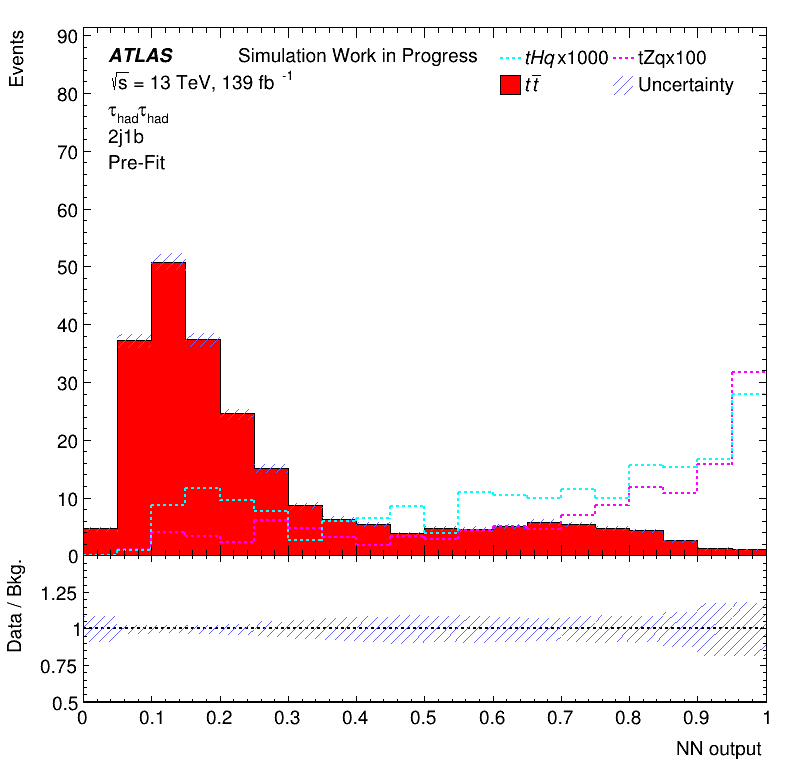
\includegraphics[width=\textwidth]{sgBkgComp}
            \end{figure}
        \end{column}
        \begin{column}{0.5\textwidth}
            \begin{itemize}
                \item \tHq against other processes
                \vspace{0.5cm}
                \item \ttbar dominates the training
                \vspace{0.5cm}
                \item \tZq misclassified as signal
                \vspace{0.5cm}
                \item Possible approaches:
                    \begin{itemize}
                        \item multiple networks
                        \item multiple targets
                        \item reweighting samples
                    \end{itemize} 
            \end{itemize}
        \end{column}
    \end{columns}
\end{frame}